%
% File acl2012.tex
%
% Contact: Maggie Li (cswjli@comp.polyu.edu.hk), Michael White (mwhite@ling.osu.edu)
%%
%% Based on the style files for ACL2008 by Joakim Nivre and Noah Smith
%% and that of ACL2010 by Jing-Shin Chang and Philipp Koehn


\documentclass[11pt]{article}
\usepackage{acl2012}
\usepackage{times}
\usepackage{latexsym}
\usepackage{amsmath}
\usepackage{multirow}
\usepackage{url}
\DeclareMathOperator*{\argmax}{arg\,max}
\setlength\titlebox{6.5cm}    % Expanding the titlebox

\title{Detecting English Writing Styles For Non Native Speakers}

\author{Rami Al-Rfou', Yanging Chen, Yejin Choi \\
  Department of Computer Science \\
  Stony Brook University \\
  NY 11794, USA \\
  {\tt \{ralrfou, cyanqing, ychoi\}@cs.stonybrook.edu}}

\date{12/15/2011}

\usepackage{graphicx}
\begin{document}
\maketitle
\begin{abstract}
%Rami's Part
%Explain what is our target of whole project.
\end{abstract}


\section{Introduction}
%Rami's Part

\section{Related Work}
%Chen's part
%Mentions what people did, and how our work is different and original.


\section{Wikipedia}
%Explain why wikipedia is an awesome source
%Explain wikipedia structure
%Explain how there are two different ways to get users contributions
%Explain the comments extraction algorithm
%Rami's Part

\section{Experiments}
%Rami's part

\subsection{Setup}
%Explain the pruning and the filtering that was done to the data.

\subsection{Popular Languages Experiment}
%Explain the experiment and the results

\begin{figure}[htp]
\centering
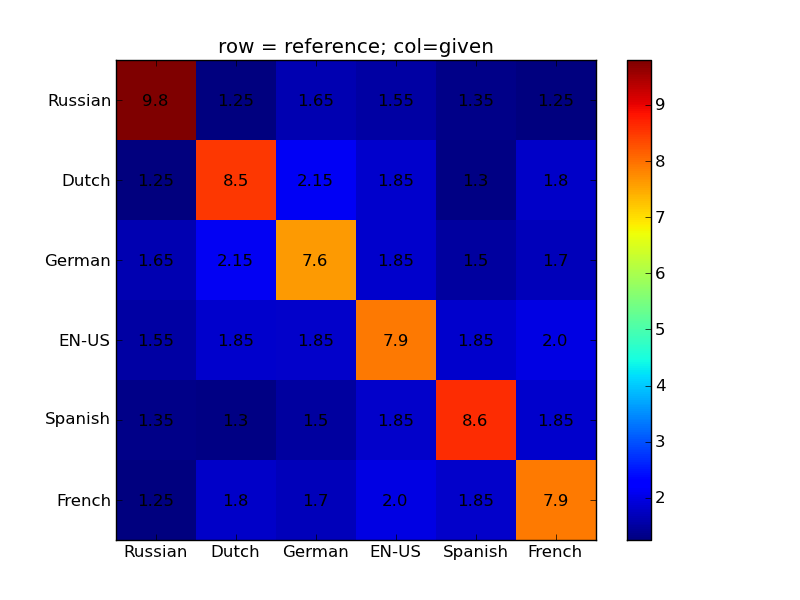
\includegraphics[scale=0.45]{popular_cfm.png}
\caption{Popular Languages experiment confusion matrix}
\label{pop_cfm}
\end{figure}
		
\subsection{Languages Families Experiment}
%Explain the experiment and the results


\subsection{Native vs Non Native Experiment}
%Explain the experiment and the results


\section{Writing Styles}
%Chen's part


\section{Conclusions}
%Chen's Part

\section*{Acknowledgments}
%Chen's Part
%We should thank Prof. Skiena for the resources he gave us.

\begin{thebibliography}{}

\bibitem[\protect\citename{Aho and Ullman}1972]{Aho:72}
Alfred~V. Aho and Jeffrey~D. Ullman.
\newblock 1972.
\newblock {\em The Theory of Parsing, Translation and Compiling}, volume~1.
\newblock Prentice-{Hall}, Englewood Cliffs, NJ.

\bibitem[\protect\citename{{American Psychological Association}}1983]{APA:83}
{American Psychological Association}.
\newblock 1983.
\newblock {\em Publications Manual}.
\newblock American Psychological Association, Washington, DC.

\bibitem[\protect\citename{{Association for Computing Machinery}}1983]{ACM:83}
{Association for Computing Machinery}.
\newblock 1983.
\newblock {\em Computing Reviews}, 24(11):503--512.

\bibitem[\protect\citename{Chandra \bgroup et al.\egroup }1981]{Chandra:81}
Ashok~K. Chandra, Dexter~C. Kozen, and Larry~J. Stockmeyer.
\newblock 1981.
\newblock Alternation.
\newblock {\em Journal of the Association for Computing Machinery},
  28(1):114--133.

\bibitem[\protect\citename{Gusfield}1997]{Gusfield:97}
Dan Gusfield.
\newblock 1997.
\newblock {\em Algorithms on Strings, Trees and Sequences}.
\newblock Cambridge University Press, Cambridge, UK.

\end{thebibliography}

\end{document}
